\documentclass[]{article}

\usepackage{graphicx}
\usepackage{amsmath}
\usepackage{textcomp}
\usepackage{geometry}
\usepackage{nicefrac}
\usepackage{siunitx}
\usepackage[english]{babel}
\usepackage[nottoc,numbib]{tocbibind}
\usepackage[autostyle]{csquotes}
\usepackage[
backend=biber,
citestyle=apa,
bibencoding=utf8,
style=apa,
sortlocale=en_US,
uniquename=false,
url=true, 
doi=true,
eprint=false
]{biblatex}
\addbibresource{./zoterolibrary.bib}
\usepackage{hyperref}
\hypersetup{colorlinks=true}
\usepackage[doublespacing]{setspace}
\usepackage{booktabs}
\usepackage{doi}
\usepackage[flushleft]{threeparttable}
\usepackage{authblk}
\usepackage[switch]{lineno}
\linenumbers
\usepackage{xr}

%\setstretch{0.75}


% NOTE: For Overleaf you need to create a latexmkrc file!
% see https://www.overleaf.com/learn/how-to/Cross_referencing_with_the_xr_package_in_Overleaf#Extra_code_for_summary.tex:_accessing_external_references
\usepackage{xfp}
\newcommand\SupplementaryMaterials{%
\xdef\presupfigures{\arabic{figure}}% save the current figure number
\xdef\presupsections{\arabic{section}}% save the current section number
\xdef\presuptables{\arabic{table}}% save the current section number
\renewcommand\thefigure{S\fpeval{\arabic{figure}-\presupfigures}}
\renewcommand\thesection{S\fpeval{\arabic{section}-\presupsections}}
\renewcommand\thetable{S\fpeval{\arabic{table}-\presuptables}}
}



\externaldocument{constrained_optimization}


\DeclareSourcemap{
\maps[datatype=bibtex, overwrite]{
% otherwise my annotations from Mendeley will be shown in the references.
\map{
\step[fieldset=annote, null]
}
% Replaces '&' with '\&'
\map{
\step[fieldsource=publisher, match=\regexp{\x{26}}, replace=\regexp{\\\x{26}}]
\step[fieldsource=journal, match=\regexp{\x{26}}, replace=\regexp{\\\x{26}}]
}
% for some reason I need this now because abstracts could contain a percentage sign and that breaks everything.
\map{
\step[fieldsource = abstract, match = \regexp{([^\\])\%}, replace = \regexp{$1\\\%}]
}
}
}


\DeclareSIUnit\year{yr}

\usepackage[font=small,labelfont=bf]{caption}

\geometry{
a4paper,
total={170mm,257mm},
left=20mm,
top=20mm,
}

\newcommand{\coo}{\ensuremath{\mathrm{CO_2}}}

\title{Supplementary Material: Reconciling the EU forest, biodiversity, and climate strategies}



\begin{document}

\author[1,*]{Konstantin Gregor}
\author[2]{Christopher P.O. Reyer}
\author[3]{Thomas A. Nagel}
\author[4, 5]{Annikki Mäkelä}
\author[1]{Andreas Krause}
\author[1]{Thomas Knoke}
\author[1]{Anja Rammig}

	\affil[1]{TUM School of Life Sciences, Technical University of Munich, Freising, Germany}
	\affil[2]{Potsdam Institute for Climate Impact Research, Member of the Leibniz Association, Potsdam, Germany}
	\affil[3]{University of Ljubljana, Department of Forestry and Renewable Forest Resources, Biotechnical Faculty, 1000 Ljubljana, Slovenia}
	\affil[4]{Department of Forest Sciences, University of Helsinki, Latokartanonkaari 7, Helsinki, Finland}
    \affil[5]{Institute for Atmospheric and Earth System Research / Forest Sciences, Faculty of Agriculture and Forestry, University of Helsinki, Finland}
	\affil[*]{Corresponding author, konstantin.gregor@tum.de}

\date{} 
\setcounter{Maxaffil}{0}

\maketitle



\newpage

\SupplementaryMaterials

\section{Supplementary Methods}

\subsection{MAXIMIN - balanced burden sharing}\label{sec:maximin}
For this approach, we simply replaced the objective function \ref{eq:sum_maxminobjective_rcp_w} with a so-called \textit{maximin} objective:

\begin{align}
	% NOTE: I removed the weights here
	\max_{\omega} & \min_{gc} \mbox{performance}(\omega^{(gc)}, gc)  +  \epsilon \sum_{gc} \mbox{performance}(\omega^{(gc)}, gc)   \label{eq:maximin_maxminobjective_rcp_w}
\end{align}

\noindent Here, the second summand is included to deal with the case where multiple solutions provide the same worst-case performance. If there are multiple such solutions, the second summand will achieve that out of these solutions, the one with the best average performance was chosen. It is important that $\epsilon$ is very small to not interfere with the optimization of the worst case, here we used $\epsilon=0.001$.
Again, without including Europe-wide constraints, the result will be the same as for the ORIGINAL and SUM optimizations.

\section{Supplementary Tables}

\begin{table}[h!]
	\small
	\caption{Comparison of our present-day (2000-2010 average) simulation outputs to results from other studies and publicly available datasets.
		The considered region is the European continent excluding Russia, Iceland, Cyprus and Malta, but including Kaliningrad region and European part of Turkey, resulting in 3124 grid cells for our simulation of which 2894 contained forest.
		Values are representative only for the forest area of this region, except for tree cover, evapotranspiration, and runoff, which are averaged over the entire region.
	}
	\label{tab:present_day}
	\begin{tabular}{llllp{18em}}
		\hline
		{} &             This study &         Literature & Data type$^{f}$ &    Reference \\
		\hline
		Vegetation carbon (PgC)                  & 13.7  &  13 & I & \textcite{Pan2011}\\
		&       &  11.7$^{a}$ & C & \textcite{ForestEurope2015} \\
		&       &  11.6$^{b}$ &  S   & \textcite{Liu2015} \\
		&       &  16.2 &  S   & \textcite{Santoro2021} \\
		Total carbon (PgC)                       & 60.4  &  40.9$^{c}$ & I & \textcite{Pan2011}\\
		Forest-GPP ($\SI{}{\gram{C}\per\year\per\square\meter}$)                       & 1263  &  1107-1199 & E, F & \textcite{Luyssaert2010}\\
		Forest-NPP ($\SI{}{\gram{C}\per\year\per\square\meter}$)                       & 502  &  447 & I & \textcite{Luyssaert2010}\\
		Fellings ($10^6\SI{}{\cubic\meter\per\year}$)         & 572   &  582 & C  & \textcite{FORESTEUROPE2020} \\
														        &    &  542 & C  & \textcite{ForestEurope2015} \\
		Total tree cover (\%)                   & 26.5  &  26.8$^{d}$ & S & GFC v1.7 Map \parencite{Hansen2013} \\
		Evapotranspiration (mm/yr)                           & 459$^{e}$   &  490 & S, M & GLEAM \parencite{Martens2016}\\
		Runoff (mm/yr)                       &  286$^{e}$  &  297 & G, M & UNH-GRDC \parencite{UNHGRDC} \\
		\hline
		\multicolumn{5}{>{\raggedright}p{\textwidth}}{$^{a}$ Using aboveground biomass = 79\% of vegetation biomass \\
			$^{b}$ Includes Turkey \\
			$^{c}$ Only upper 100cm  of soil considered (we consider 150cm) \\
			$^{d}$ Tree cover here refers to canopy closure for all vegetation taller than $\SI{5}{\meter}$ (GFC) and LPJ-GUESS simulated crown cover of all simulated forests. GFC contains tree cover also for non-forest areas \\
			$^{e}$ Assuming C3 grass growing everywhere outside of forest areas \\
			$^{f}$ Data source meanings: S - satellite-derived, I - inventory data, C - country reporting, M - modelled, G - Gauge-observations, F - flux measurements from ecological site, E - ecological site studies
		}
		
		
	\end{tabular}
\end{table}














\section{Supplementary Figures}



\begin{figure}[!h]
	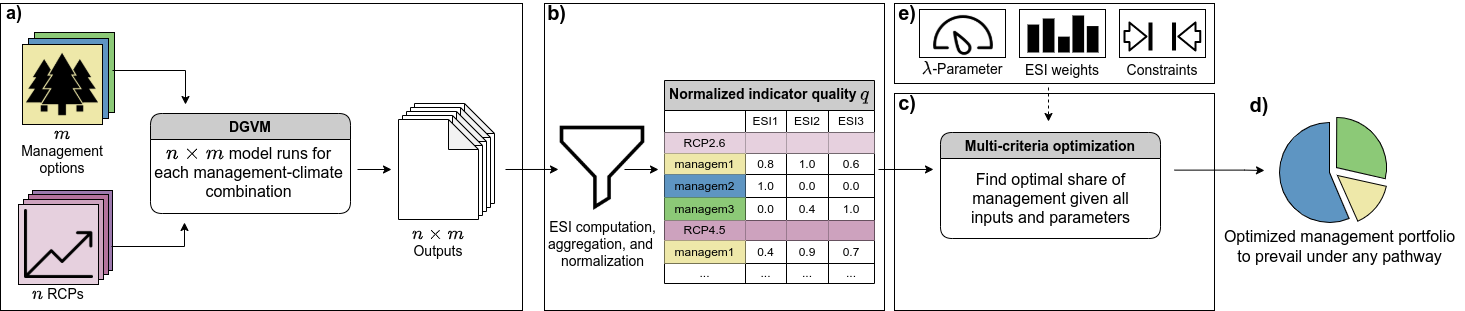
\includegraphics[width=\linewidth]{supplement_figs/optimization.png}
	\caption{Schematic visualization of the \textit{default-opt} methodology, which computes one single portfolio independently per grid cell. 
		\textbf{a)} For the \textit{m} management options and \textit{n} RCPs, $n\times m$ model simulations are conducted. 
		\textbf{b)} ESIs are derived from model outputs, aggregated to the 2100-2130 mean, and normalized. Thus for each grid cell, there was one table containing the normalized values for all RCPs and management options. 
		\textbf{c)} The optimization computes \textbf{d)} one optimized portfolio. This ensures a balanced provision of all ESIs across all RCPs. 
		\textbf{e)} The parameter $\lambda \in [0, 1]$ specifies the focus on the balanced provision of the ESI. A low $\lambda$ focuses more on a balanced provision of ESIs while a high $\lambda$ improves more the average ESI performance (see section \ref{sec:original-optimization}). ESI weights were not considered in this study. Additional constraints can put bounds on the optimization. Figure from \textcite{Gregor2022}.
	}
	\label{fig:optimization}
\end{figure}



\begin{figure}
	\centering
	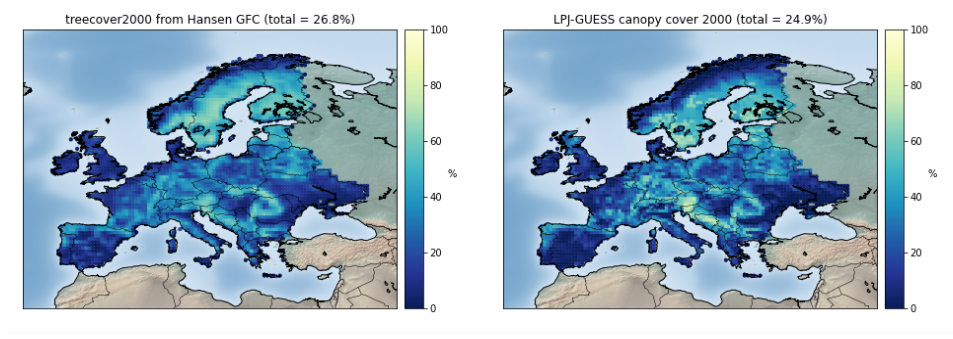
\includegraphics[width=0.7\linewidth]{supplement_figs/poultervshansen}
	\caption{Comparison of the tree cover dataset of \parencite{Hansen2013} (left; upsampled bi-linearly to match the 0.5° resolution) and the LPJ-GUESS modeled canopy cover (right; based on the prescribed forest areas per grid cell of \parencite{poulter2018tgfa}.}
	\label{fig:poultervshansen}
\end{figure}





\begin{figure}[h!]
	\centering
	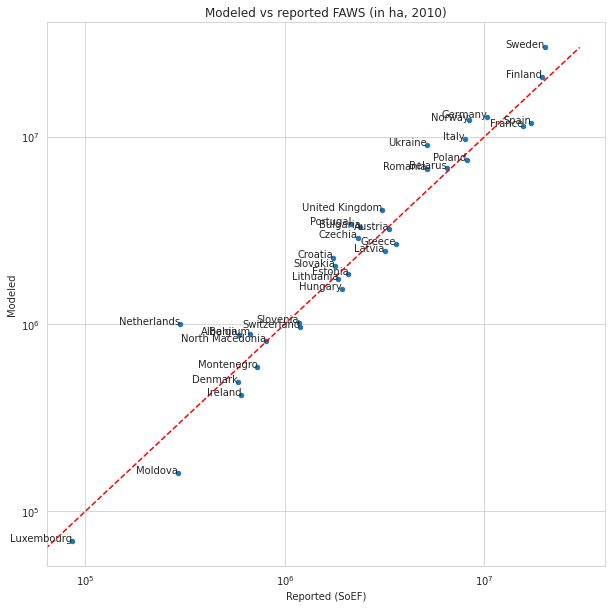
\includegraphics[width=\linewidth]{supplement_figs/evalutation_faws.png}
	\caption{Evaluation of the modeled area of forests available for wood supply compared to recent estimates for the year 2010 \parencite{FORESTEUROPE2020}.}
	\label{fig:eval-faws}
\end{figure}




\begin{figure}[h!]
	\centering
	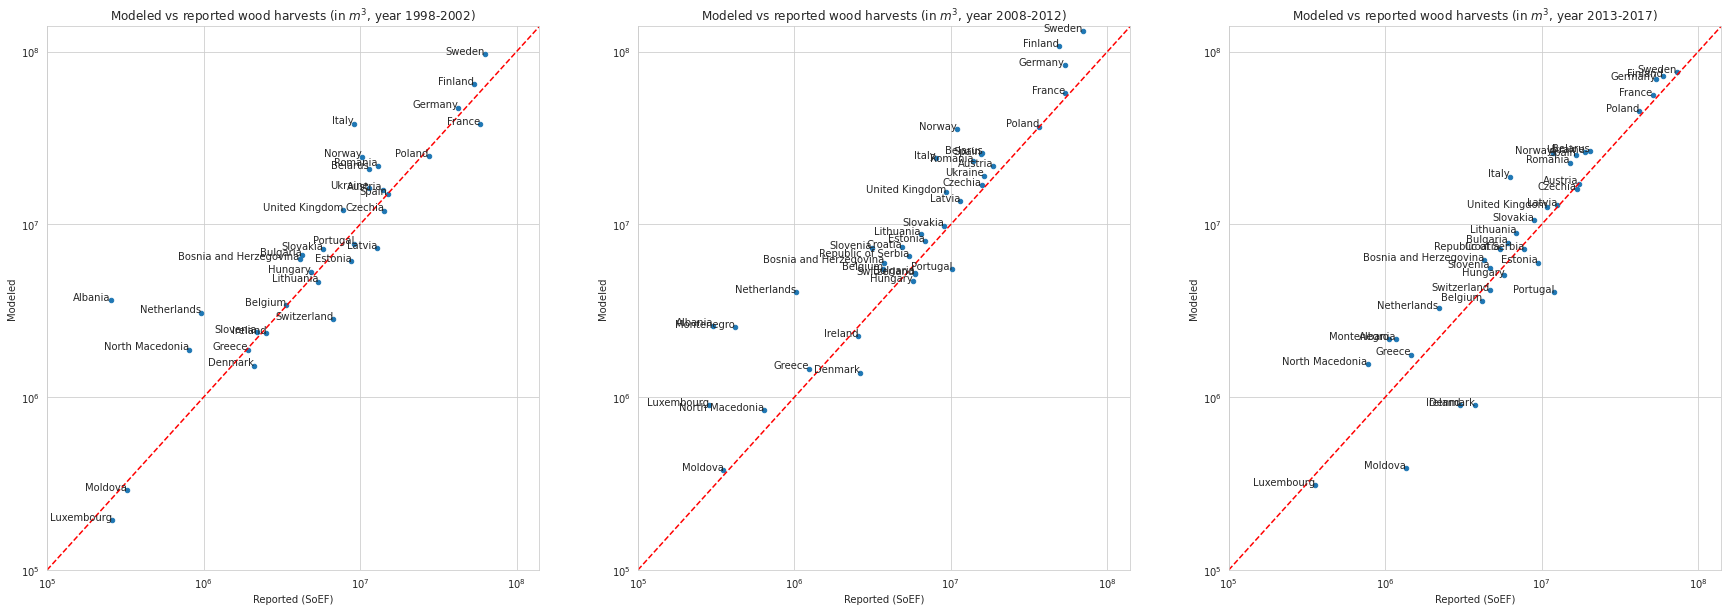
\includegraphics[width=\linewidth]{supplement_figs/evalutation_wood_harv.png}
	\caption{Evaluation of the modeled volumes of wood harvests compared to recent estimates for the years 2000, 2010, and 2015 \parencite{FORESTEUROPE2020}.}
	\label{fig:eval-harvest-country}
\end{figure}




\begin{figure}[!h]
	\centering
	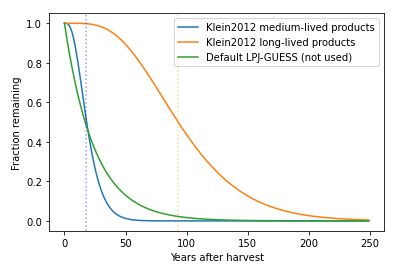
\includegraphics[width=0.5\linewidth]{supplement_figs/gamma_functions.png}
	\caption{Decay functions for each wood product pool based on Gamma distributions \parencite{Klein2013}. Scale and shape parameters for the long-lived (medium-lived) pool are 19.3 and 5.15 (5.52 and 3.68), respectively. This method accounts for a time lag between the creation of a product and its decay. Median residence times are indicated by dashed vertical lines.}
	\label{fig:gamma}
\end{figure}





\begin{figure}[h!]
	\centering
	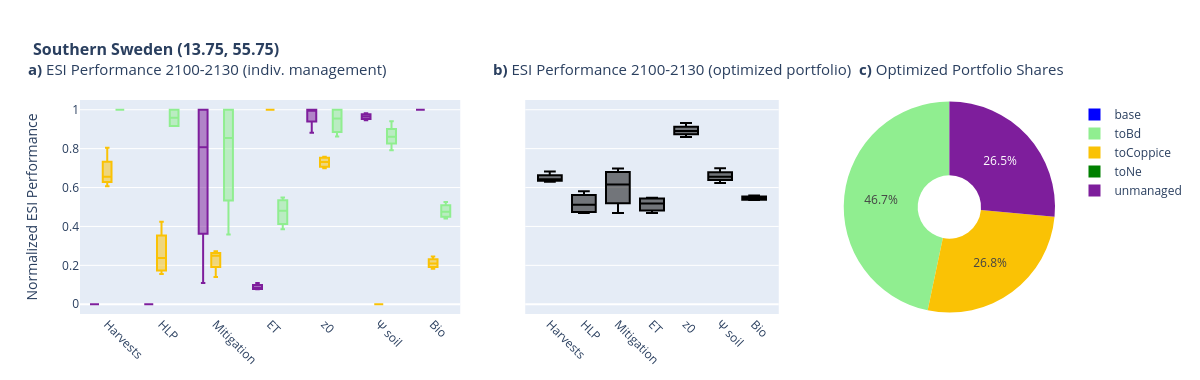
\includegraphics[width=0.9\linewidth]{supplement_figs/balanced_gridcell.png}
	\caption{Application of the \textit{default-opt optimization} for a sample grid cell in Sweden. management options may be beneficial for some ecosystem services and bad for others (e.g., unmanaged forests are simulated to be good for biodiversity but they are obviously bad for harvests). management options also may be either good or bad for an ecosystem service, depending on the RCP: \textbf{a)} E.g., unmanaged forests are good for mitigation in a low-emission world, because mitigation is dominated by the carbon sink in the forest. But they might be bad for mitigation in a high-emission world in which the substitution effect of wood products has an important impact on mitigation. This is indicated by the spread over the y-axis. The optimized portfolio in \textbf{c)}, however, provides all ecosystem services in an optimally balanced way \textbf{(b)}. Figure taken from \textcite{Gregor2022}}
	\label{fig:balanced-gridcell}
\end{figure}





\begin{figure}[!h]
	\centering
	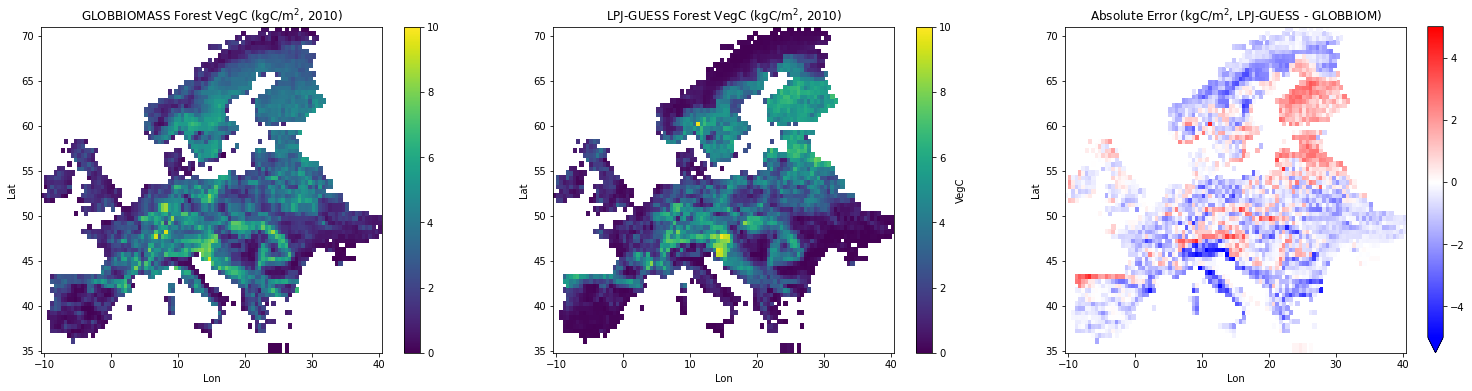
\includegraphics[width=0.9\linewidth]{supplement_figs/vegC_vs_globbiom.png}
	\caption{Modeled vegetation carbon compared to recent estimates of \textcite{Santoro2021}.}
	\label{fig:vegc}
\end{figure}



















%%%%%%%%%%%%%%%%%%%%%%%%%%%%%%%%%%%%%%%%%%%%%%
%%%%%%%%%%%%%%%%%%%%%%%%%%%%%%%%%%%%%%%%%%%%%%
% END MODEL EVAL
%%%%%%%%%%%%%%%%%%%%%%%%%%%%%%%%%%%%%%%%%%%%
%%%%%%%%%%%%%%%%%%%%%%%%%%%%%%%%%%%%%%%%%%%%







\begin{figure}[h!]
	\centering
	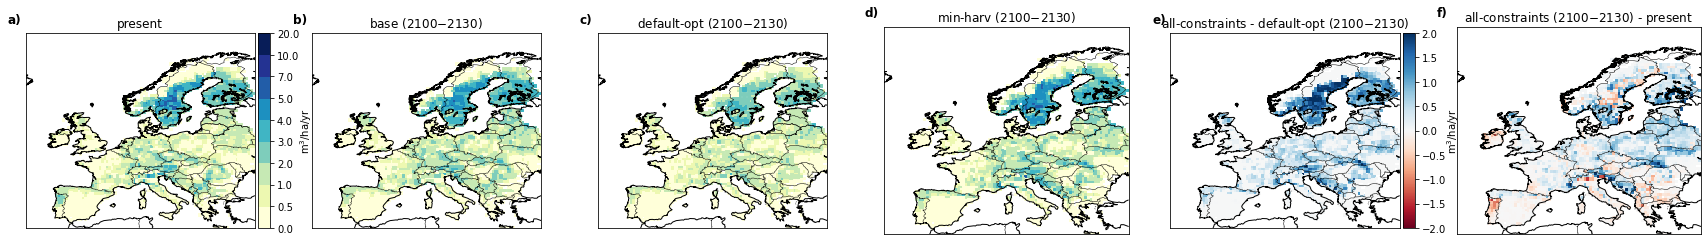
\includegraphics[width=\linewidth]{supplement_figs/harvest_provision_sum_default_maintain_harv45.png}
	\caption{Modeled harvest provision (in $\SI{}{\cubic\meter\per\hectare\per\year}$ dry biomass) \textbf{a)} at present-day ), \textbf{b)} in the future for RCP4.5, when current forest composition remains stable, \textbf{c)} after optimizing without constraints (\textit{default-opt}), and \textbf{d)} when imposing the harvest constraint (\textit{min-harv}). e) and f) show the difference of \textit{min-harv} and \textit{default-opt} and present day, respectively. The difference between the two optimizations in \textbf{e)} shows that in Southern Scandinavia, a lot more wood was harvested in the constrained optimization compared to the default optimization.}
	\label{fig:harvest-provision}
\end{figure}



\begin{figure}[h!]
	\centering
	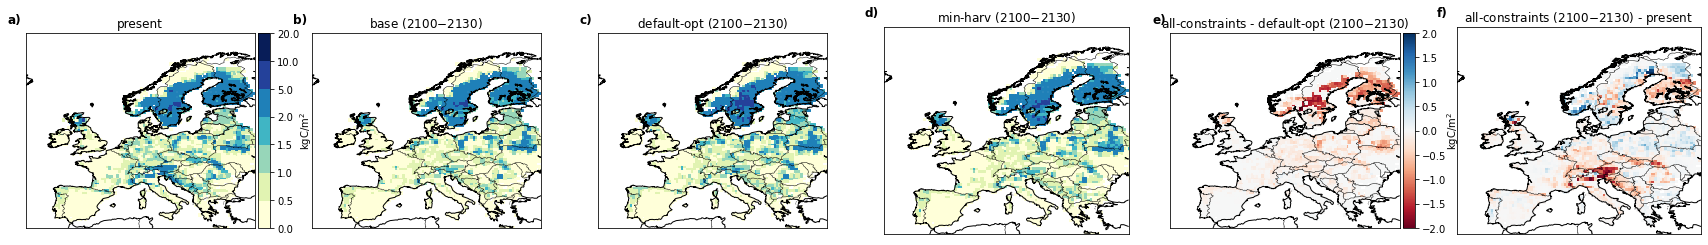
\includegraphics[width=\linewidth]{supplement_figs/cwd_provision_sum_default_maintain_harv45.png}
	\caption{Amount of coarse woody debris \textbf{a)} at present-day, \textbf{b)} in the future for RCP4.5, when current forest composition remains stable, \textbf{c)} after optimizing without constraints (\textit{default-opt}), and \textbf{d)} when imposing the harvest constraint (\textit{min-harv}). e) and f) show the difference of \textit{min-harv} and \textit{default-opt} and present day, respectively. The difference between the two optimizations in \textbf{e)} shows how the harvest constraint decreases the available coarse woody debris especially in Scandinavia, compared to the \textit{default-opt} portfolios, where large share of the region are unmanaged, leading to a larger amount of coarse woody debris compared to \textit{min-harv} where the region is heavily managed.}
	\label{fig:cwd}
\end{figure}



\begin{figure}[h!]
	\centering		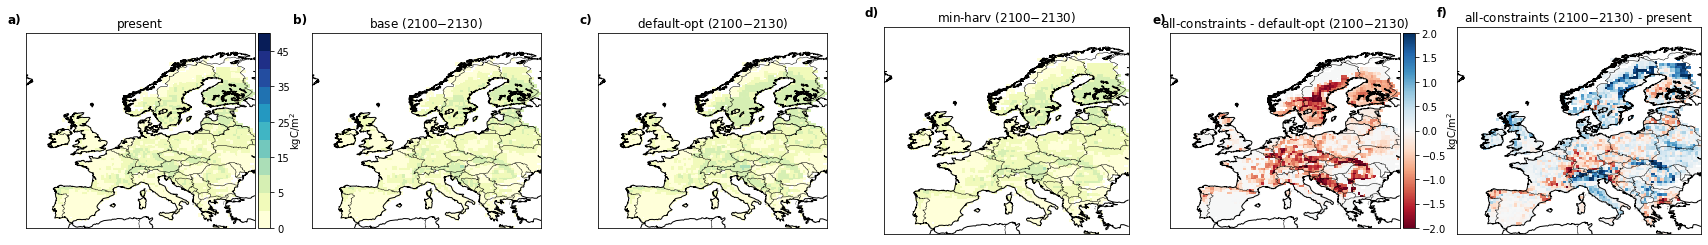
\includegraphics[width=\linewidth]{supplement_figs/cpool_provision_sum_default_maintain_harv45.png}
	\caption{Same as Fig. \ref{fig:cwd} but for the total carbon pool in the forest (vegetation + deadwood + soil)}
	\label{fig:cpool}
\end{figure}





\begin{figure}[h!]
	\centering		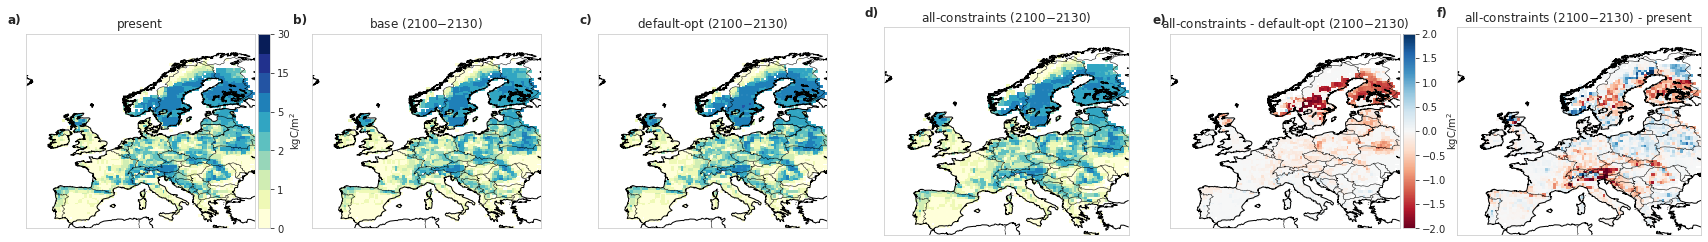
\includegraphics[width=\linewidth]{supplement_figs/cpool_provision_sum_default_all_litter45.png}
	\caption{Same as Fig. \ref{fig:cwd} but for the entire litter carbon pool in the forest.}
	\label{fig:litter45}
\end{figure}


\begin{figure}[h!]
	\centering		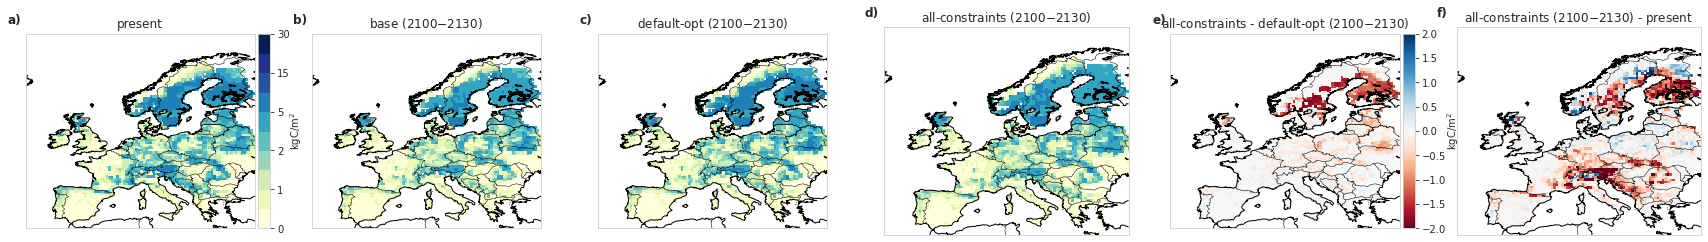
\includegraphics[width=\linewidth]{supplement_figs/cpool_provision_sum_default_all_litter85.png}
	\caption{Same as Fig. \ref{fig:litter45} but for RCP8.5.}
	\label{fig:litter85}
\end{figure}


\begin{figure}[h!]
	\centering		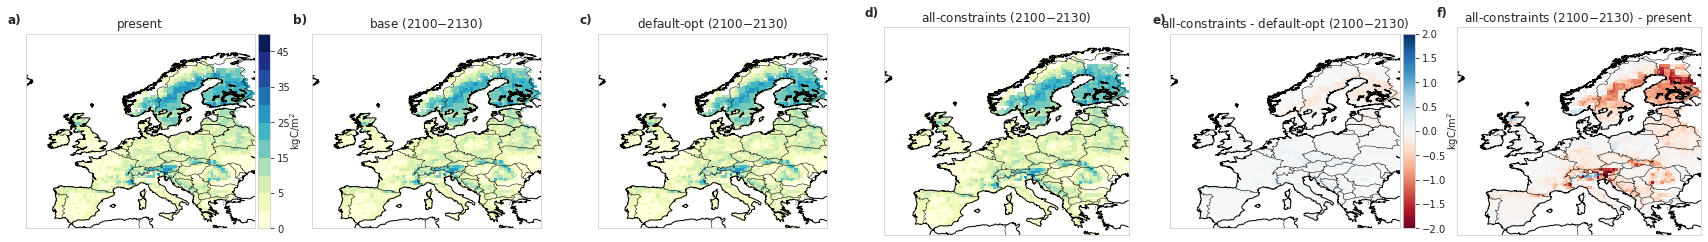
\includegraphics[width=\linewidth]{supplement_figs/cpool_provision_sum_default_all_soil45.png}
	\caption{Same as Fig. \ref{fig:cwd} but for the soil carbon pool in the forest.}
	\label{fig:soil45}
\end{figure}




\begin{figure}[h!]
	\centering		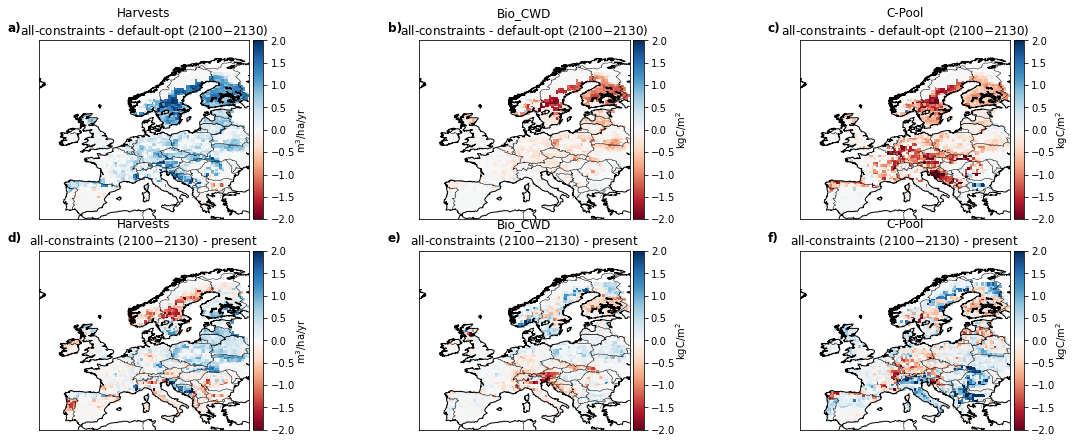
\includegraphics[width=\linewidth]{supplement_figs/es_provision_diffs26.png}
	\caption{Same as Fig. \ref{fig:es-provision-diffs} but for RCP2.6.}
	\label{fig:es-provision-diffs26}
\end{figure}



\begin{figure}[h!]
	\centering		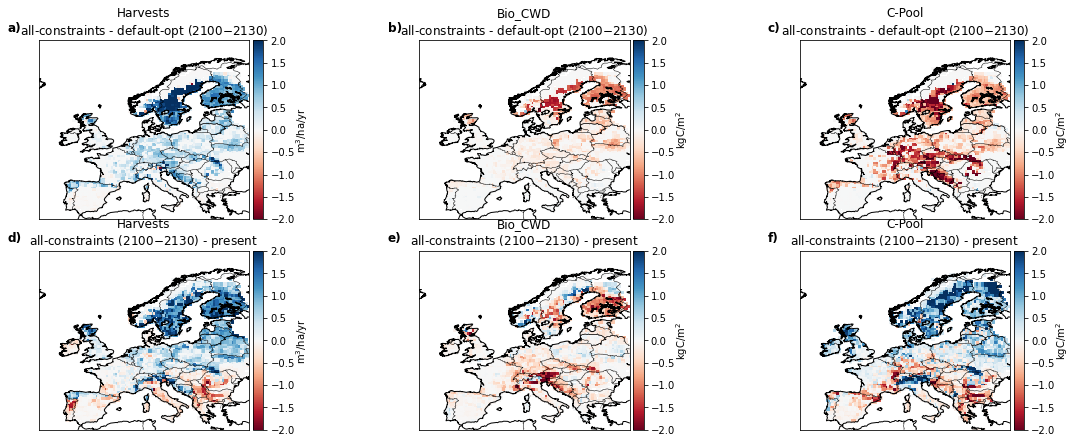
\includegraphics[width=\linewidth]{supplement_figs/es_provision_diffs85.png}
	\caption{Same as Fig. \ref{fig:es-provision-diffs} but for RCP8.5.}
	\label{fig:es-provision-diffs85}
\end{figure}


\begin{figure}[h!]
	\centering
	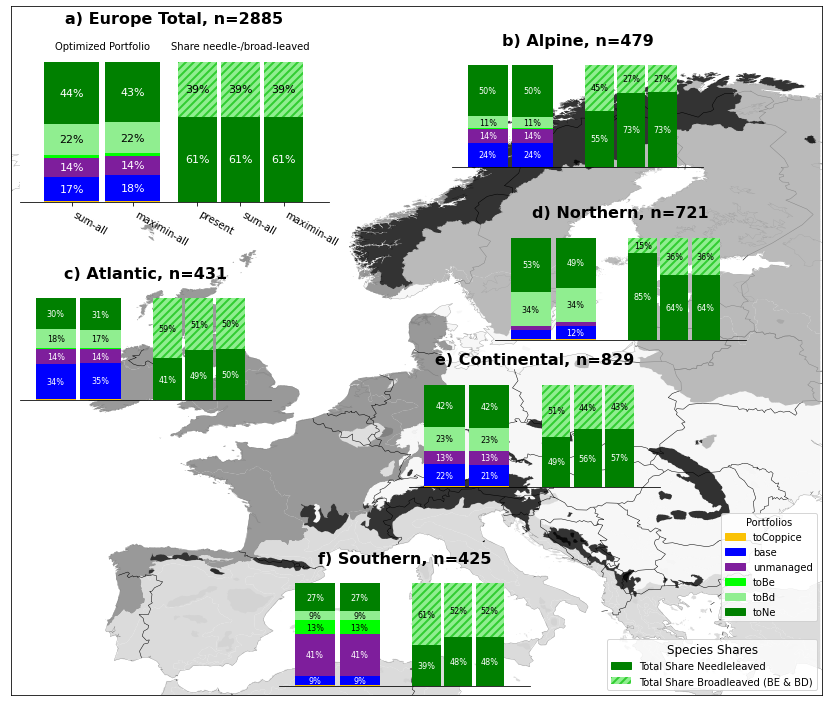
\includegraphics[width=0.9\linewidth]{supplement_figs/sum_vs_minmax_all.png}
	\caption{Optimized portfolios for \textit{all-constraints} for the SUM- and the MAXIMIN-method. There are only marginal differences between the two results. This highlights the limited options to optimize ecosystem service provision.}
	\label{fig:sum-vs-minmax}
\end{figure}





\begin{figure}[h!]
	\centering
	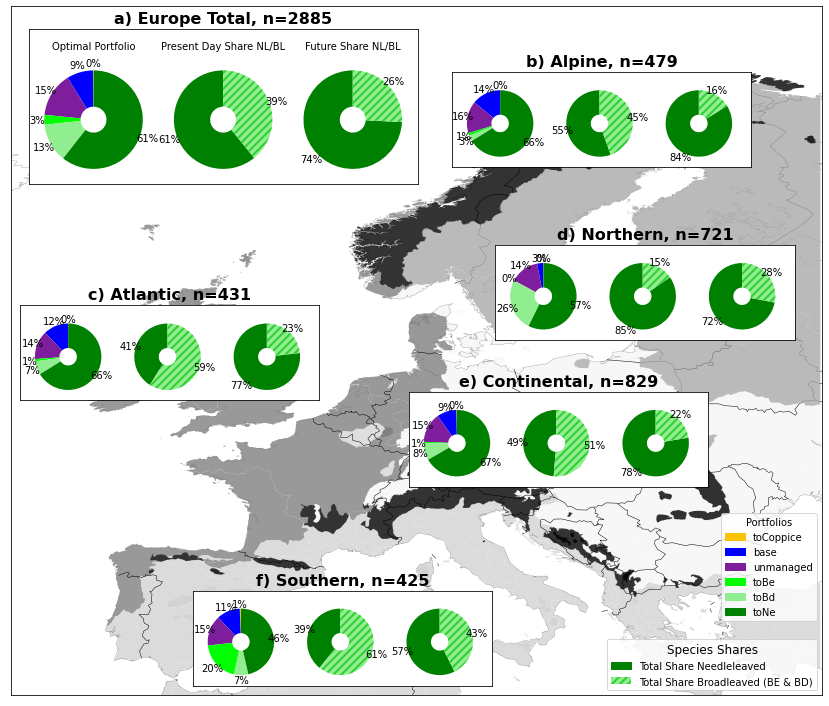
\includegraphics[width=0.9\linewidth]{supplement_figs/unmanaged_cell_high_ne.png}
	\caption{When relaxing the harvest constraint by allowing a decrease of 5\% in harvests, the optimizer finds a solution where the share of unmanaged forests is provided in every grid cell. However, this leads to a tremendous focus on needle-leaved forests, conflicting with current science and policies that foster broad-leaved and mixed forests due to their higher resilience to climate change.}
	\label{fig:unmanaged-cell}
\end{figure}



\begin{figure}[h!]
	\centering
	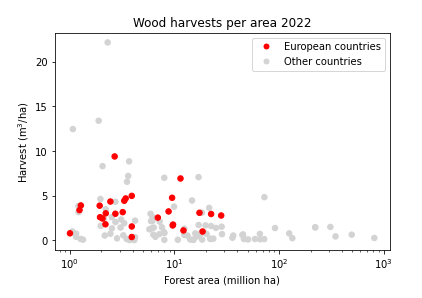
\includegraphics[width=0.75\linewidth]{supplement_figs/fao_wood_harvests_europe_vs_rest.png}
	\caption{Wood harvests per area are rather high in European countries compared to the rest of the world. Note the log-scale of the x-axis and that countries with less than 1 million ha of forests were excluded. Graphic: own, data source: \textcite{FAOSTAT2022}.}
	\label{fig:faowoodharvest}
\end{figure}



\clearpage

\printbibliography[title=Supplementary References]


\end{document}

